\documentclass{beamer}
\usetheme[block=fill]{metropolis}

\usepackage[english]{babel}
%\usepackage[utf8]{inputenc}

% For notes
\usepackage{pgfpages}
\setbeameroption{show notes on second screen=right}
\usepackage{appendixnumberbeamer} % don't number the backup slides

\usepackage{amsmath,amssymb} % math
\usepackage{graphicx} % images
\DeclareGraphicsExtensions{.eps,.pdf,.png,.jpg,.gif}
\graphicspath{{./img/}}

\title{aursec - A blockchain approach to securing software packages}
\author{Lukas Krismer \& Bennett Piater}
\institute{Universität Innsbruck - QE - Christian Sillaber}
\date{\today}

\begin{document}

\maketitle


\begin{frame}
	\frametitle{Outline}
	\tableofcontents
	\note{1 min L}
\end{frame}

\section{AUR}

\begin{frame}{AUR}
\begin{itemize}
	\item \textbf{AUR}=\alert{A}rch Linux \alert{U}ser \alert{R}epository
	\item Contains package build scripts (PKGBUILDs)
	\item Packages can be voted for inclusion in the official repositories
	\item Easy to use using so-called AUR helpers
	\item Everybody can upload PKGBUILDs
	\item Anyone can adopt orphaned packages
\end{itemize}
\note{2min L}
\end{frame}

\begin{frame}{Threat Assessment}
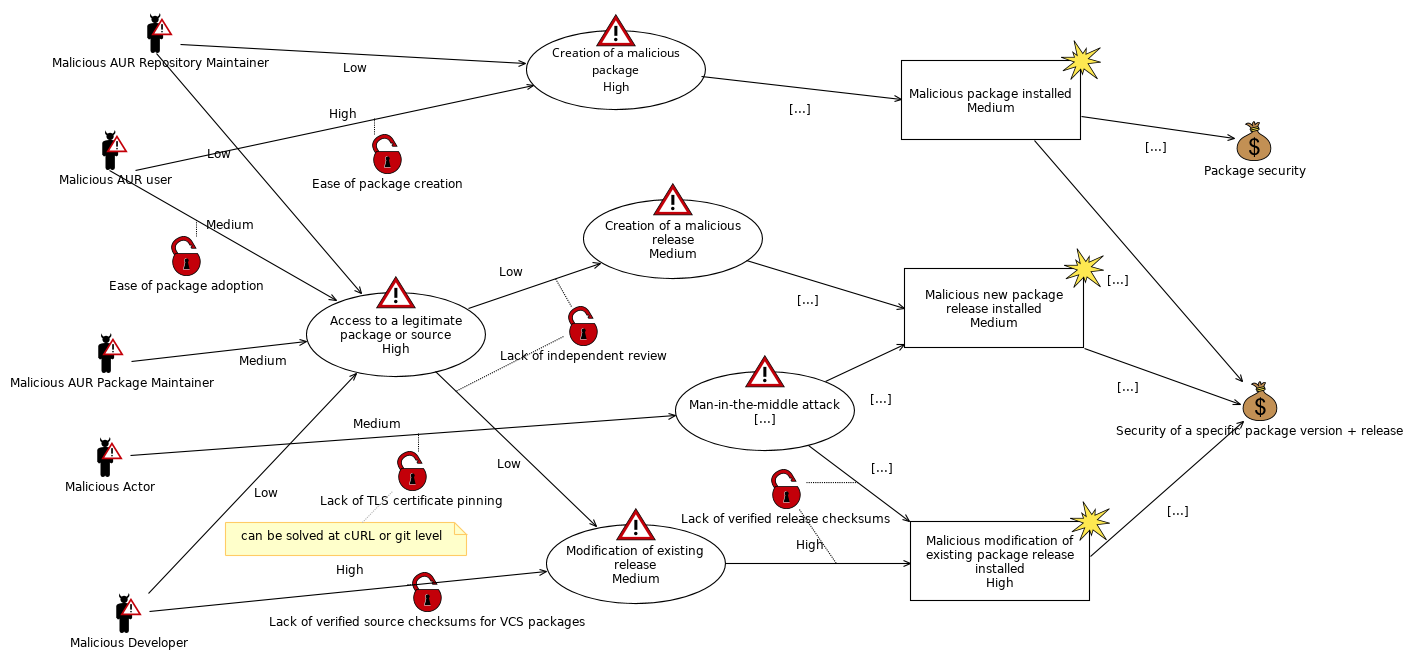
\includegraphics[width=\textwidth]{threat.png}
\note{2 min B}
\end{frame}

\section{Our Project}

\begin{frame}{Covered Threats}
\includegraphics<1>[width=\textwidth]{threat.png}
\includegraphics<2>[width=\textwidth]{threat.png} %TODO: change to reworked threatdiag.
\note{1 min L}
\end{frame}

\begin{frame}{Basic Workflow of the Core Library}
%\icludegraphics[width=\textwidth]{bennets.diagram}
\note{3 min L}
\end{frame}

\begin{frame}{Components}
\begin{itemize}
	\item Program on a private Ethereum blockchain
	\item Library and program using it
	\item AUR package
	\item Integration in aurutils
	\item Threat analysis of the AUR and our software
	\item Web- and/or CLI-Interface for stats
\end{itemize}
\note{2 min B}
\end{frame}

\begin{frame}{Schedule}
\begin{itemize}
	\item \textbf{25.10} \emph{prototype:} hashing \hfill B
	\item \textbf{08.11} \alert{Initial Presentation}\hfill L
	\item \textbf{15.11} \emph{prototype:} library without blockchain back-end \hfill B/L
	\item \textbf{15.11} Bash-API for the blockchain \hfill L
	\item \textbf{30.11} \emph{finish:} \alert{Solidity program} \hfill B
	\item \textbf{08.12} deploy local blockchain for development \hfill L
	\item \textbf{08.12} running server with ethereum-node \hfill B/L
	\item \textbf{15.12} \emph{prototype:} \alert{Library} incl. back-end \hfill L
	\item \textbf{20.12} \emph{contrib:} rudimentary pre-build-hooks in aurutils \hfill B
\end{itemize}
\note{2 min B}
\end{frame}

\begin{frame}{Schedule}
\begin{itemize}
	\item \textbf{10.01} \emph{contrib:} TLS-public-key-pinning in aurutils \hfill B
	\item \textbf{10.01} configuration and trust-cutoff \hfill L
	\item \textbf{15.01} \emph{test:} \alert{Integration in aurutils} \hfill B
	\item \textbf{15.02} \alert{AUR package} incl. private blockchain \hfill B
	\item \textbf{01.03} \emph{finish:} libary and aurutils-Hook \hfill B
	\item \textbf{01.04} \emph{finish:} Web- and/or CLI-Interface \hfill L
	\item \textbf{15.04} \alert{Draft paper} \hfill
	\item \textbf{??.05} \emph{finish:} Paper\hfill
	\item \textbf{??.05} Final presentation\hfill L
\end{itemize}
\note{2 min B}
\end{frame}


\end{document}
